\section{Synthesis}
Finally, the VHDL design has been synthesized for the ZyBo board. This section
reports the main metrics: timing, power and utilization.

\subsection{Timing}
\begin{center}\vspace*{\baselineskip}
    \def\arraystretch{1.5}
    \begin{tabular}{|c|c|}\hline
        \textbf{Setup Worst Negative Slack (WNS)} & 57.119\si{\nano\second}\\\hline
        \textbf{Setup Total Negative Slack (TNS)} & 0.000\si{\nano\second}\\\hline
        \textbf{Worst Hold Slack (WHS)} & 0.215\si{\nano\second}\\\hline
        \textbf{Total Hold Slack (THS)} & 0.000\si{\nano\second}\\\hline
    \end{tabular}\vspace*{\baselineskip}
\end{center}

Since the clock frequency was set at 16\si{\mega\hertz}, the critical path 
is $62.5-57.119 = 5.381 \si{\nano\second}$ long and therefore the maximum operating
frequency is $1/5.381 \simeq 185 \si{\mega\hertz}$. However, there is no point 
in going too fast since it would just increase the power consumption (samples come 
in at a 16\si{\kilo\hertz} rate).

The critical path is represented by the multiplier that is used to square the 
sample, hence using the approximated absolute value brings no benefit to timing.

\subsection{Power}
The power report has been generated in Vivado using the default settings.

\begin{center}\vspace*{\baselineskip}
    \def\arraystretch{1.5}
    \begin{tabular}{|c|c|}\hline
        \textbf{Total On-Chip Power} & 0.09\si{\watt}\\\hline
        \textbf{Junction Temperature} & 26.0\si{\celsius}\\\hline
        \textbf{Thermal Margin} & 59.0\si{\celsius} (5.0\si{\watt})\\\hline
        \textbf{Effective $\theta$\si{\joule\ampere}} & 11.5\si{\celsius/\watt}\\\hline
        \textbf{Power supplied to off-chip devices} & 0\si{\watt}\\\hline
        \textbf{Confidence level} & Low\\\hline
    \end{tabular}\vspace*{\baselineskip}
\end{center}

\begin{figure}[h!]
    \centering
    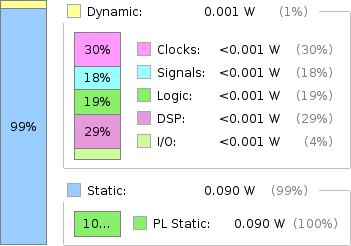
\includegraphics[width=0.75\textwidth]{figs/power_report_master.png}
    \caption{Power report}
    \label{fig:power_master}
\end{figure}

\subsection{Utilization}
\begin{center}\vspace*{\baselineskip}
    \def\arraystretch{1.5}
    \begin{tabular}{|c|c|c|c|c|}\hline
        \textbf{Resource} & \textbf{Utilization} & 
        \textbf{Utilization ``opt''} & \textbf{Difference} & 
        \textbf{Available}\\\hline
        LUT & 118  (0.67\%) & 110   (0.63\%) & \textbf{8} & 17600 \\\hline
        FF  &  74  (0.21\%) &  73   (0.21\%) & \textbf{1} & 35200 \\\hline
        DSP &   1  (1.25\%) &   1   (1.25\%) & 0          &    80 \\\hline
        IO  &  20 (20.00\%) &  20  (20.00\%) & 0          &   100 \\\hline
    \end{tabular}\vspace*{\baselineskip}
\end{center}

From the utilization we can see how 8 LUTs would be saved if we used the 
approximation of the absolute value.

\subsection{Warnings}
{\footnotesize
\begin{verbatim}
[Constraints 18-5210] No constraints selected for write.
Resolution: This message can indicate that there are no constraints for the 
design, or it can indicate that the used_in flags are set such that the 
constraints are ignored. This later case is used when running synth_design to 
not write synthesis constraints to the resulting checkpoint. Instead, project 
constraints are read when the synthesized design is opened.
\end{verbatim}
}

Constraints were correctly set, thus this might be a bug of Vivado. 
In fact, timing report works fine with the set timing constraints.

{\footnotesize
\begin{verbatim}
NSTD #1 Critical Warning 
20 out of 20 logical ports use I/O standard (IOSTANDARD) value 'DEFAULT', 
instead of a user assigned specific value. This may cause I/O contention or 
incompatibility with the board power or connectivity affecting performance, 
signal integrity or in extreme cases cause damage to the device or the 
components to which it is connected. To correct this violation, specify all I/O
standards. This design will fail to generate a bitstream unless all logical 
ports have a user specified I/O standard value defined. To allow bitstream 
creation with unspecified I/O standard values (not recommended), use this 
command: set_property SEVERITY {Warning} [get_drc_checks NSTD-1].  
NOTE: When using the Vivado Runs infrastructure (e.g. launch_runs Tcl command), 
add this command to a .tcl file and add that file as a pre-hook for 
write_bitstream step for the implementation run. Problem ports: x[15], x[14], 
x[13], x[12], x[11], x[10], x[9], x[8], x[7], x[6], x[5], x[4], x[3], x[2], x[1] 
(the first 15 of 20 listed). 
\end{verbatim}
}

I/O mapping was not set since it should be done by whom integrates the VAD 
component with his own project.

{\footnotesize
\begin{verbatim}
DPIP #1 Warning 
DSP squarepowernet_component/n_sq_repr input squarepowernet_component/n_sq_repr/A[29:0] 
is not pipelined. Pipelining DSP48 input will improve performance. 
\end{verbatim}
}

Pipeline registers have already been added.

{\footnotesize
\begin{verbatim}
ZPS7 #1 Warning 
The PS7 cell must be used in this Zynq design in order to enable correct default
configuration. 
\end{verbatim}
}

The PS7 block probably refers to the ARM Processor environment, thus is not required
in our design.\footnote{\url{https://forums.xilinx.com/t5/Welcome-Join/How-to-instantiate-the-PS7-block/m-p/333953\#M4847}}.